\chapter{Aplicação operacional e TUI}\label{aplicauxe7uxe3o-operacional-e-tui}

A aplicação constitui parte do produto do TCC e não apenas uma interface auxiliar. Seu papel é tornar executável, auditável e reproduzível a sequência completa de extração, validação, treinamento e comparação dos modelos. A interface atual é uma TUI baseada em Rich, executada em ambiente Python gerenciado por \texttt{uv}.

\section{Filosofia da TUI}\label{filosofia-da-tui}

A TUI mantém a lógica de negócio nos módulos Python e utiliza a interface apenas como orquestrador. Isso preserva duas formas de execução: interativa, para engenharia e pesquisa, e CLI, para automação ou depuração. A mesma operação disparada pelo menu pode ser reproduzida por comando de terminal.

O menu principal agrupa as funções operacionais de geração de dados, modelagem, auditoria e investigação. A organização documentada da interface inclui:

\begin{verbatim}
[1] Gerar Dataset
[2] Treinar & Validar Modelos
[3] Visualizar Estatísticas do Data Lake
[4] Comparar Especialistas vs Modelo Global
[5] Minerar Evidências de Anomalias e Sub-Clusters
[6] Abrir Cockpit Analítico Web
[7] Executar Auditoria de Saúde e Testes
[8] Configurações Globais
[9] Sair
\end{verbatim}

\section{Geração do dataset}\label{gerauxe7uxe3o-do-dataset}

A opção de geração de dataset oferece quatro modos: cidade completa em um dia de referência, alimentador específico, período histórico e sincronização inteligente. Em todos eles o operador escolhe o formato de saída (\texttt{parquet}, \texttt{csv} ou ambos) e acompanha a fila de lotes do MDM.

No modo de sincronização inteligente, a aplicação consulta a cobertura já existente no Data Lake e determina automaticamente quais dias precisam ser extraídos. Se houver lacuna interna, ela também entra na fila. Esse comportamento transforma a extração em processo idempotente: repetir o comando não significa repetir o trabalho concluído.

Durante a execução, cada \emph{worker} apresenta estado individual - aguardando, consultando Oracle, recebendo registros, normalizando ou gravando - além da barra de progresso global. O desenho favorece diagnóstico de gargalos e evita que uma execução longa pareça um processo opaco.

\section{Estatísticas e calendário do Data Lake}\label{estatuxedsticas-e-calenduxe1rio-do-data-lake}

A opção de estatísticas apresenta dimensões das camadas, distribuição por alimentador e um calendário mensal de continuidade. O usuário pode auditar ambos os formatos ou selecionar apenas Parquet ou CSV. Dias completos, parciais e ausentes são distinguidos visualmente.

A mesma área permite sincronizar formatos faltantes. Uma partição disponível apenas em Parquet pode ser convertida para CSV e vice-versa sem reconsultar o Oracle. Essa funcionalidade reduz custo de banco e separa claramente \textbf{aquisição} de \textbf{formatação para consumo}.

\section{Auditoria de saúde e testes}\label{auditoria-de-sauxfade-e-testes}

A auditoria executa validações estruturais e a suíte de testes do projeto. O relatório diário registra a condição do Data Lake e deve atuar como \emph{gate} anterior ao treinamento. Um modelo não deve ser treinado simplesmente porque arquivos existem; as camadas precisam satisfazer os contratos mínimos esperados.

Entre os controles relevantes estão: schemas, chaves, presença das partições, consistência de datas, cardinalidade dos joins, histórico UC--NIO e disponibilidade dos atributos exigidos. Esse estágio reduz o risco de treinar modelos sobre datasets silenciosamente degenerados.

\section{Ordem de treinamento}\label{ordem-de-treinamento}

A TUI organiza o treinamento em níveis. A ordem representa dependências metodológicas e permite comparação controlada, sem pressupor que todas as técnicas tenham contribuição marginal positiva.

\begin{figure}
\centering
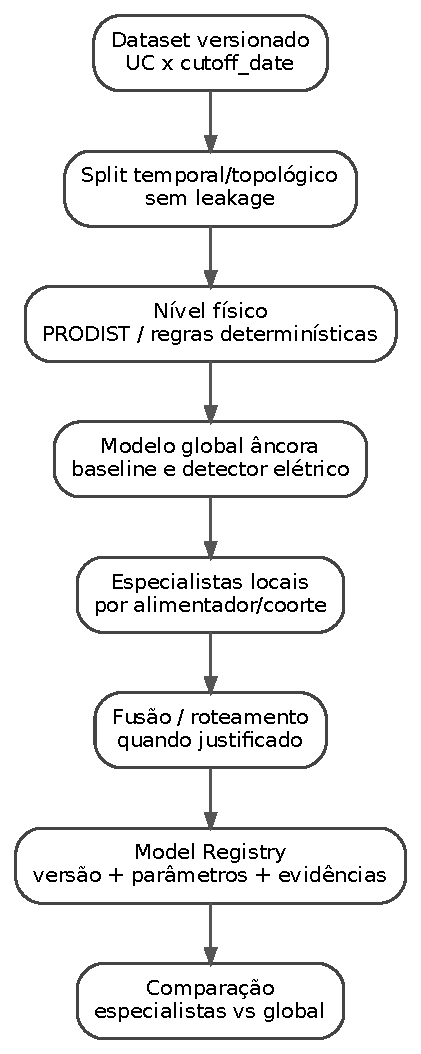
\includegraphics[width=0.94\textwidth,height=0.65\textheight,keepaspectratio]{figures/training_order.pdf}
\caption{Ordem operacional de treinamento e governança.}\label{fig:training}
\par\small Fonte: elaboração própria.
\end{figure}

A ordem ilustrada na Figura \ref{fig:training} é uma ordem de dependências analíticas: qualidade antes de inferência elétrica, referência comportamental antes de comparação local e contexto antes de decisão de campo. Ela não deve ser interpretada como demonstração de que todas as etapas foram validadas com inspeções; representa sequência reproduzível de construção e testes.

O primeiro nível contém regras e classificadores físicos. O segundo contém os modelos de comportamento e anomalia: modelo global, especialistas locais por alimentador e arquitetura multivisão. A fusão ou roteamento entre especialistas é avaliada somente depois que o desempenho de cada componente isolado é conhecido. Um baseline simples permanece como referência para impedir que maior complexidade seja confundida com melhoria.

A unidade canônica de modelagem é \texttt{UC~x~cutoff\_date}. Identificadores (\texttt{id\_\_}) e metadados de controle (\texttt{meta\_\_}) são separados dos atributos (\texttt{x\_\_}) e dos futuros rótulos (\texttt{y\_\_}). Transformações que aprendem parâmetros são ajustadas somente no conjunto de treino, e o split deve respeitar temporalidade e agrupamentos para reduzir vazamento temporal \autocite{geron2025}.

\section{Especialistas locais e distribuição por alimentador}\label{especialistas-locais-e-distribuiuxe7uxe3o-por-alimentador}

A possibilidade de treinar por alimentador tem dois objetivos. O primeiro é científico: verificar se populações topologicamente mais homogêneas produzem limites e arquétipos mais estáveis. O segundo é operacional: permitir que a equipe examine um circuito específico sem reprocessar a cidade inteira.

O modelo local não substitui automaticamente o modelo global. A avaliação deve comparar ambos no mesmo recorte e adotar o local somente quando houver volume suficiente e benefício mensurável. Caso contrário, o modelo global funciona como âncora.

\section{Model Registry e comparação de versões}\label{model-registry-e-comparauxe7uxe3o-de-versuxf5es}

Cada treinamento deve gerar uma versão identificável, associada ao intervalo de dados, catálogo de atributos, parâmetros, seed e código. O Model Registry permite comparar versões e impedir que a última execução seja automaticamente tratada como a melhor.

A TUI oferece comparação entre especialistas e modelo global no conjunto de teste, respeitando os contratos de cada experimento. A comparação deve ser acompanhada não somente por métricas clássicas, mas também por estabilidade do ranking, cobertura da população, número de UCs encaminhadas a cada fila e impacto operacional.

\section{Configurações globais e reprodutibilidade}\label{configurauxe7uxf5es-globais-e-reprodutibilidade}

Parâmetros operacionais como formato de saída, \emph{random state} e taxa de contaminação podem ser alterados pela interface. Para o trabalho científico, essas configurações devem ser persistidas junto ao experimento. O ambiente é gerenciado com \texttt{uv}, reduzindo divergência de dependências entre execuções.

Credenciais de bancos não fazem parte do código ou dos artefatos científicos. A aplicação utiliza configuração externa por ambiente ou arquivo local ignorado pelo controle de versão.

\section{Protótipo de Cockpit e perspectiva de integração operacional}\label{protuxf3tipo-de-cockpit-e-perspectiva-de-integrauxe7uxe3o-operacional}

A TUI permanece orientada à engenharia do pipeline. O protótipo funcional do painel web possui finalidade diferente: consumir resultados já processados, filtrar a carteira, acompanhar indicadores e abrir o detalhe de cada UC. A consulta temporal sob demanda permite examinar o recorte de interesse sem carregar toda a população de uma vez.

A interface analítica foi concebida para apresentar filtros de alimentador, período, categoria, escore e status operacional; presets de investigação; seleção dinâmica de colunas; exportação de listas; e um painel de detalhe contendo série temporal, evidências por especialista, regras acionadas, topologia, histórico do NIO. A associação com o status de inspeção é uma extensão futura.

A distinção entre as interfaces é, portanto, complementar: a \textbf{TUI} destina-se a executar, auditar, treinar e governar os experimentos, enquanto a \textbf{interface Web} destina-se a interpretar, priorizar e acompanhar os resultados computacionais.

\section{Cobertura funcional completa da TUI e interfaces associadas}\label{cobertura-funcional-completa-da-tui-e-interfaces-associadas}

A TUI baseada em Rich foi concebida como interface de operação da pesquisa, sobretudo nos ambientes onde comandos de terminal são mais adequados do que uma aplicação gráfica pesada. O menu reúne extração, treinamento, governança do Data Lake, comparação de modelos, mineração de evidências, abertura do Cockpit, diagnóstico de saúde e configuração. A capacidade de inspecionar a disponibilidade dos dados antes de executar o treino é parte do método de controle de qualidade, e não somente uma facilidade de interação.

\begin{longtable}[]{@{}
  >{\raggedright\arraybackslash}p{(\columnwidth - 4\tabcolsep) * \real{0.3333}}
  >{\raggedright\arraybackslash}p{(\columnwidth - 4\tabcolsep) * \real{0.3333}}
  >{\raggedright\arraybackslash}p{(\columnwidth - 4\tabcolsep) * \real{0.3333}}@{}}
\caption{Funcionalidades da interface de terminal}\label{tab:integracao5}\\
\toprule\noalign{}
\begin{minipage}[b]{\linewidth}\raggedright
Recurso
\end{minipage} & \begin{minipage}[b]{\linewidth}\raggedright
Entrada ou escolha
\end{minipage} & \begin{minipage}[b]{\linewidth}\raggedright
Resultado e significado operacional
\end{minipage} \\
\midrule\noalign{}
\endfirsthead
\toprule\noalign{}
\begin{minipage}[b]{\linewidth}\raggedright
Recurso
\end{minipage} & \begin{minipage}[b]{\linewidth}\raggedright
Entrada ou escolha
\end{minipage} & \begin{minipage}[b]{\linewidth}\raggedright
Resultado e significado operacional
\end{minipage} \\
\midrule\noalign{}
\endhead
\bottomrule\noalign{}
\endlastfoot
Extração por \texttt{days\_back} & um dia relativo & reprocessamento pontual e comparação de artefatos \\
Intervalo histórico & datas inicial/final & recuperação de janelas e composição do histórico \\
Auto-backfill & calendário e horizonte temporal & identificação de dias ausentes e atualização incremental \\
Filtro por alimentador & nome/identificador topológico & execução local e comparação com população global \\
Formato de saída & Parquet, CSV ou ambos & persistência tipada e intercâmbio para inspeção \\
Progresso por worker & lotes em execução & acompanhamento de gargalos, consultas e falhas \\
Calendário mensal & partições diárias e canais & observação de datas ausentes e formatos parciais \\
Auditoria de contagens & tabelas e períodos & inspeção da cardinalidade e divergências \\
Sincronização de formatos & Parquet e CSV & recuperação de cópias sem nova consulta à fonte \\
Treinamento baseline & matriz temporal de atributos & referência comparativa IF/K-Means \\
Treinamento composto & atributos elétricos & consenso entre detectores e regras \\
Treinamento hierárquico & dataset e alimentador & modelos locais, escore global e roteamento \\
Classificador de tensão & dados/etiquetas de referência & experimento auxiliar de classificação elétrica \\
Filtro temporal de treino & janela selecionada & controle de corte e repetibilidade \\
Registro de modelos & artefatos e métricas & versionamento e comparação de versões \\
Comparação especialista/global & mesmo conjunto de teste & análise de diferenças de decisão \\
Health audit & diretórios e manifestos & identificação de falhas e inconsistências \\
Hiperparâmetros & contaminação, seed, formato & execução controlada e reprodutível \\
\end{longtable}
{\small\noindent Fonte: elaboração própria.\par}


A Tabela \ref{tab:integracao5} cobre os comandos documentados da TUI e esclarece que algumas operações são orquestradas pela interface enquanto outras dependem de scripts externos. O pipeline completo com meteorologia é um caminho de pesquisa por linha de comando, não uma opção necessariamente presente no menu. De forma semelhante, a existência de uma opção de \emph{Model Registry} não garante que toda governança de modelos esteja automatizada; o registro e a comparação precisam ser distinguidos das interfaces parciais e de futuras decisões de promoção de versões.

O calendário fornece dois diagnósticos diferentes que devem ser apresentados juntos: o \textbf{estado materializado da partição} e a \textbf{completude efetiva da telemetria}. Um dia com Parquet presente pode continuar contendo lacunas para uma parcela dos NIOs; uma falha de conversão entre formatos não equivale a ausência do evento no MDM. A visualização permite decidir se a ação correta é converter uma cópia, reextrair um dia, inspecionar o vínculo UC--NIO ou encaminhar medidores ao especialista de comunicação.

A comparação de modelos deve ocorrer sobre o mesmo corte, mesma coorte elegível e mesmos atributos, exceto pela alteração deliberada no ablation study. Sem esse controle, variações na correlação de postos (Spearman), na sobreposição de carteiras (Jaccard Top-$K$) ou no volume de alertas podem decorrer apenas de alterações na amostra avaliada. Ao salvar o modelo, o repositório de artefatos deve ser interpretado em conjunto com o manifesto de dados e o pré-processamento correspondente.

A aplicação Web complementa a TUI, mas atende outro usuário: o analista que precisa investigar a UC no tempo. Seu Raio-X apresenta curva de energia, referência histórica, indicador de cobertura, categoria e evolução da anomalia, com consulta temporal sob demanda e navegação entre candidatos. Uma eventual posição na lista deve remeter ao mesmo instante de corte e à mesma versão de modelo registrada pela execução de treinamento; do contrário, TUI e Cockpit exibiriam decisões de campanhas distintas sem identificação.


A interface de terminal organizou extração, treinamento, governança do armazenamento, comparação de modelos, diagnóstico de saúde e configuração. O calendário reuniu informações sobre partições, formatos e datas. A investigação pôde distinguir uma cópia ausente em certo formato de um dia sem dados na origem. O registro da versão do modelo, período de ajuste, semente e atributos permitiu associar a inferência à configuração correspondente.

O painel web permitiu consultar a UC, examinar uma janela de energia, comparar o histórico com a referência e inspecionar cobertura e categoria. A tela por UC e a visão de carteira respondem a perguntas diferentes. Na primeira, o analista investiga o instante e a natureza do desvio. Na segunda, seleciona uma população por período e contexto e verifica sua prioridade relativa.

Os indicadores do consolidado exploratório (referência histórica de 20/11) contaram 66.099 UCs distintas, 262.849 janelas e 932 UCs com o indicador binário de anomalia no último corte disponível por unidade (além de 274 UCs marcadas como candidatas à vistoria nessa mesma base). Em contraste, a campanha \texttt{OOT\_MULTIVIEW} (6.037 candidatas na execução consolidada de 25/11) e a série \texttt{DAILY\_RULES} (4.978 candidatas em 19/11) operam sob políticas de limiar e regras de triagem próprias no corte final. Uma seleção baseada em categoria diagnóstica, um escore acima do limiar e a presença na fila final são operações distintas que exigem especificar regra, data de corte e denominador.






\section{Leitura operacional da hierarquia e dos casos}
A TUI consulta a hierarquia cadastral de 69.895 UCs. Nesse universo, o circuito F-03 reúne 9.278 UCs e 5.290 estão sem alimentador. A distribuição exploratória do Capítulo~\ref{anuxe1lise-exploratuxf3ria-do-conjunto-de-dados} considera as 66.099 UCs do consolidado: 8.810 no maior circuito e 4.694 sem alimentador. Para reproduzir uma contagem é necessário manter a mesma população e a mesma chave de agregação.

\begin{figure}[htbp]\centering\caption{Inventário das camadas e hierarquia cadastral na interface de terminal}\label{fig:tui-auditoria-menu}
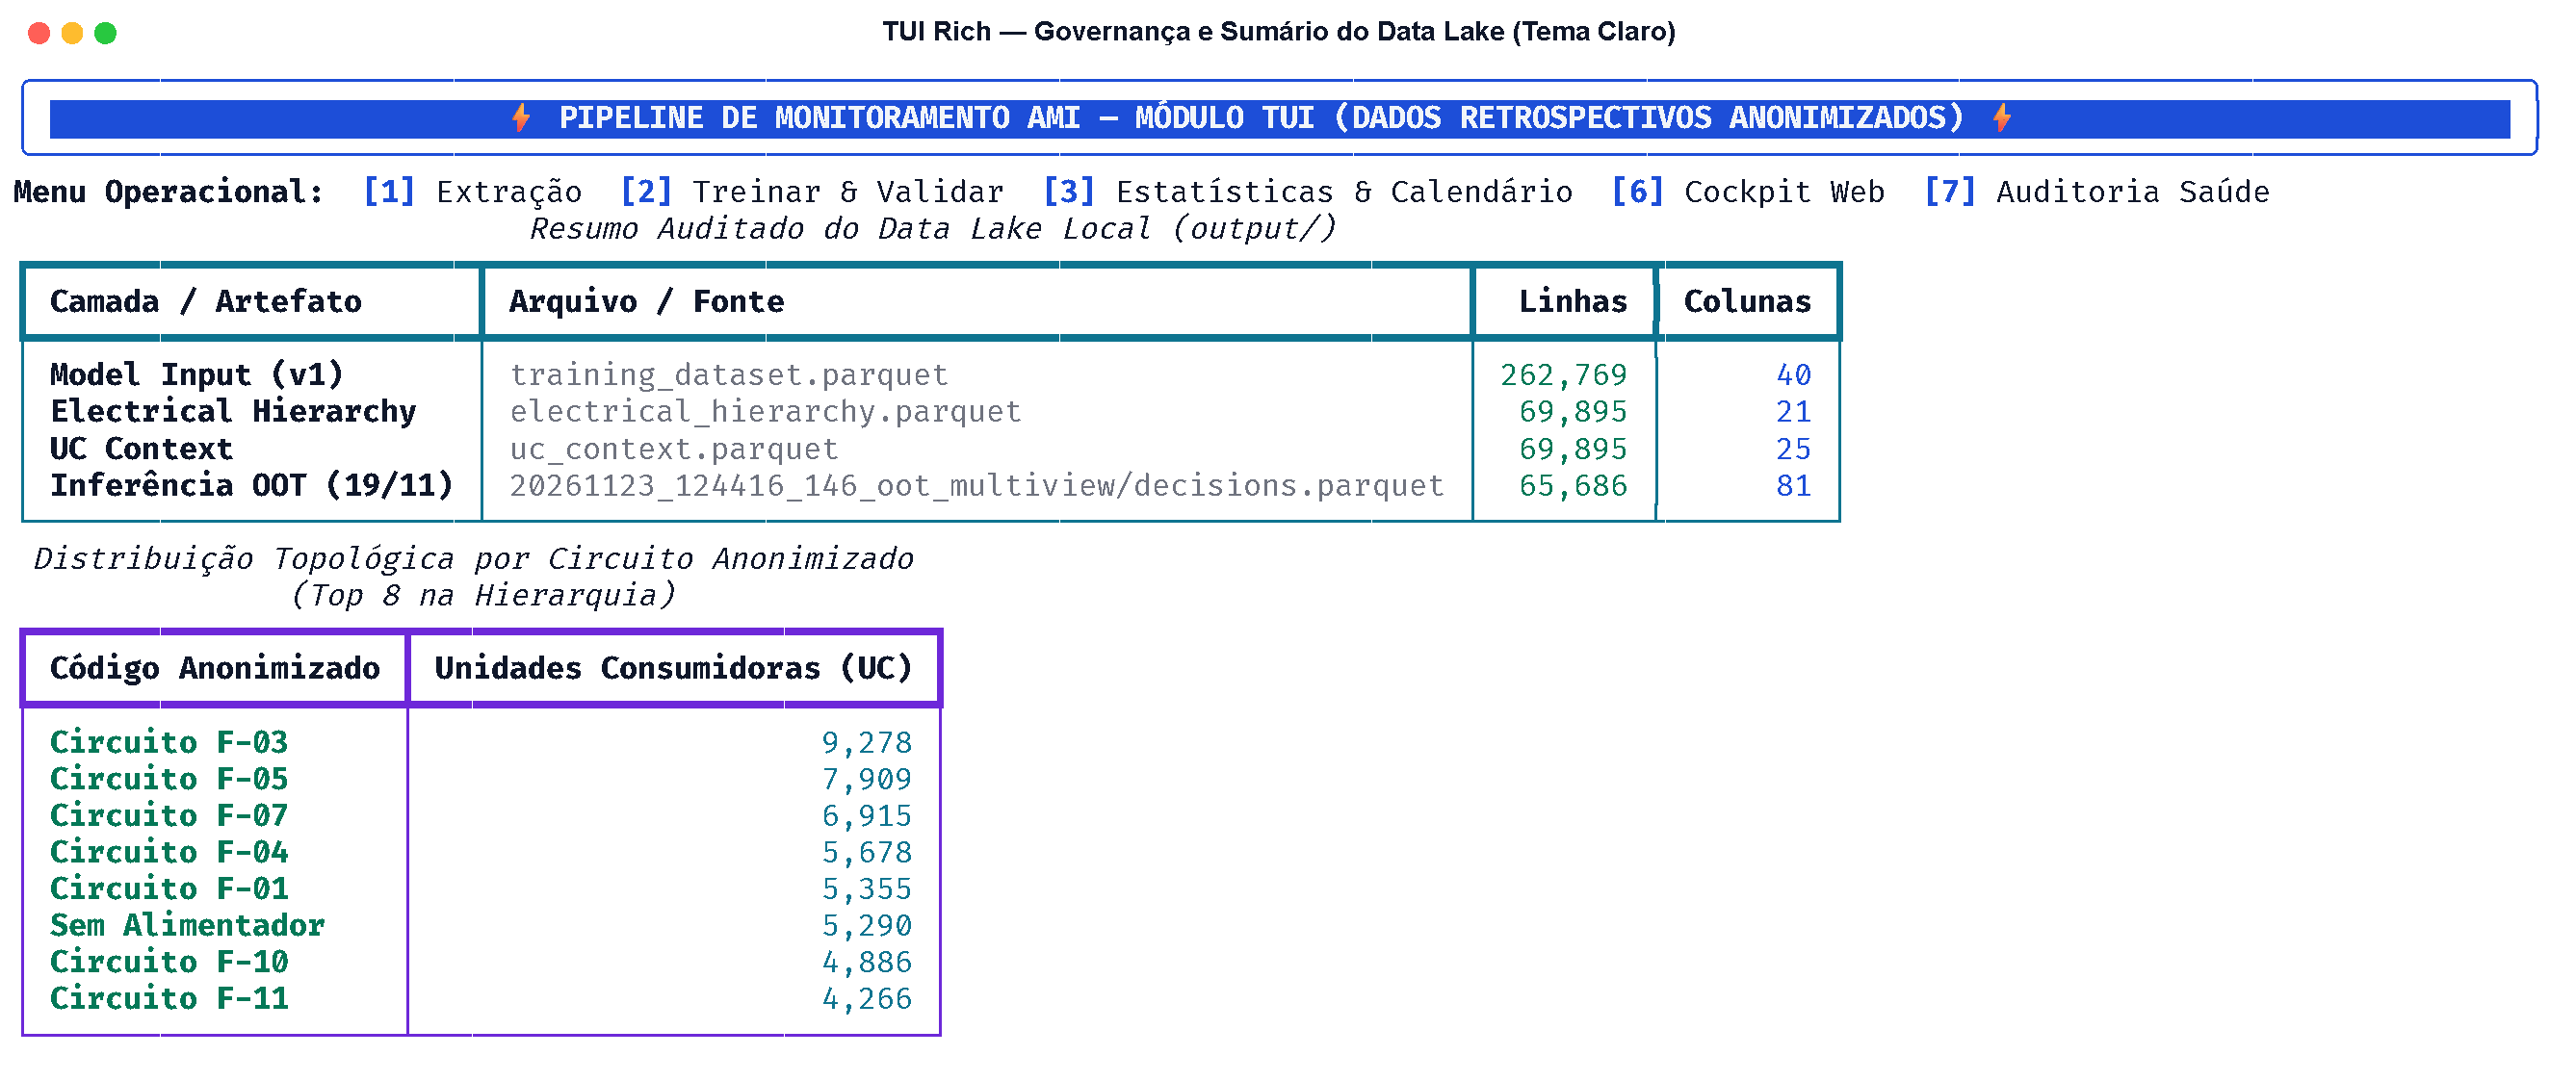
\includegraphics[width=.96\linewidth,height=.44\textheight,keepaspectratio]{figuras/fig_4_4a_tui_menu_governanca.pdf}
\par\small Fonte: elaboração própria, inventário da interface em 23/11. O arquivo de treino tinha 262.769 linhas nessa captura, 80 a menos que as 262.849 janelas do consolidado exploratório.
\end{figure}

Na consulta individual da UC 908***00, há dois intervalos temporais distintos. A telemetria esteve ausente em 29 e 30/10. De 31/10 a 19/11 transcorreram 20 dias de calendário, incluindo os extremos. A janela que começa no primeiro dia de silêncio totaliza 22 dias. A decisão OOT final registra 17 no contador de dias consecutivos de anomalia. A Figura~\ref{fig:caso-908xxx00-completo} preserva as lacunas da série de energia e exibe a cobertura correspondente.
